\documentclass[preview]{standalone}

\usepackage[english]{babel}
\usepackage{amsmath}
\usepackage{amssymb}

\usepackage[svgnames]{xcolor}
\usepackage{tikz}
\usetikzlibrary{calc}
\tikzstyle{zero}=[circle,draw=black,fill=white,inner sep=0pt,minimum size=2.5mm]	\tikzstyle{one}=[circle,draw=black,fill=black,inner sep=0pt,minimum size=2.5mm]	\tikzstyle{two}=[circle,draw=black,fill=gray,inner sep=0pt,minimum size=2.5mm] 
\begin{document}

\begin{align*}
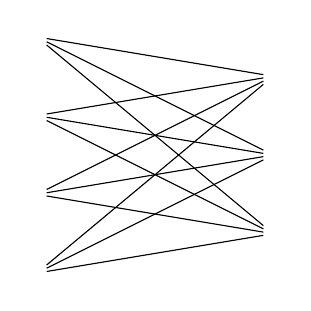
\begin{tikzpicture}\foreach \t in {1,2,3,4}	{\node  (\t) at  (1,\t) {};}\foreach \t/\l in {1/A,2/B,3/C} {\node (\l) at  (4,\t+.5) {};}\foreach \x in {1,2,3,4}\foreach \l in {A,B,C} \filldraw(\x)--(\l);\end{tikzpicture}
\end{align*}

\end{document}
